\section{Binarna reakcija}

V binarni reakciji ob trku dveh molekul A nastane en radikal $\text{A}^*$, ki nato razpade na molekuli B in C:
\begin{align}
    2\, A \, &\autorightleftharpoons{p}{q} \, A + A^* \\ \nonumber
    A^* \, &\autorightarrow{r}{} \, B+C
\end{align}

Hitrosti reakcij popišemo s spodnjimi tremi NDE, kjer v aproksimaciji stacionarnega stanja velja $\dot{[\text{A}^*]} \approx 0$.
\begin{align}
    \dot{[\text{A}]} &= 2\,q\,[\text{A}] - p\,[\text{A}]^2 \\ \nonumber
    \dot{[\text{A}^*]} &= p\,[\text{A}]^2 - q\,[\text{A}]\,[\text{A}^*] - r\,[\text{A}^*] \\ \nonumber
    \dot{[\text{B}]} = \dot{[\text{C}]} &= r\,[\text{A}^*]
\end{align}
Pri deljenju s $p$ se sistem poenostavi na le dva parametra $\alpha = q/p$ in $\beta = r/p$. Tako znaša razmerje $r/q = \beta / \alpha$.
\begin{align}
    \dot{[\text{A}]} &= 2\, \alpha \,[\text{A}] - [\text{A}]^2 \\ \nonumber
    \dot{[\text{A}^*]} &= [\text{A}]^2 - \alpha \,[\text{A}]\,[\text{A}^*] - \beta \,[\text{A}^*] \\ \nonumber
    \dot{[\text{B}]} = \dot{[\text{C}]} &= \beta \,[\text{A}^*]
\end{align}
V primeru aproksimacije stacionarnega stanja tako iz zgornjega izraza za $\dot{[\text{A}^*]}$ dobimo
\begin{equation}
    [\text{A}^*] = \frac{[\text{A}]^2}{\alpha \, [\text{A}] + \beta}
\end{equation}

Ob začetni koncentraciji $A(0) = 1$ in $q/p = 1000$ za različna razmerja $r/q$ dobimo različne hitrosti poteka reakcije, ki pa ne vpliva na končno stanje, kar je prikazano na sliki \ref{fig:zahtevani_izrač}. Na sliki \ref{fig:napaka_stacionarnega} pa je prikazano, kaj se zgodi, ako obrnemo preferenčno smer 1.reakcije, torej ustrezno zmanjšamo razmerje $q/p = 1/1000$. Tedaj je reakcija 1000x hitrejša v desno smer, zato nastane tudi vršna koncentracija $\text{A}^*$, na koncu pa se vzpostavi enako ravnovesje. Pri tem opazimo, da naša aproksimacija stacionarnega stanja ne velja več, saj se je močno povečala koncentracija $\text{A}^*$, ki je bila pri primerih na sliki \ref{fig:zahtevani_izrač} sicer ustrezna.
\begin{figure}[H]
    \centering
    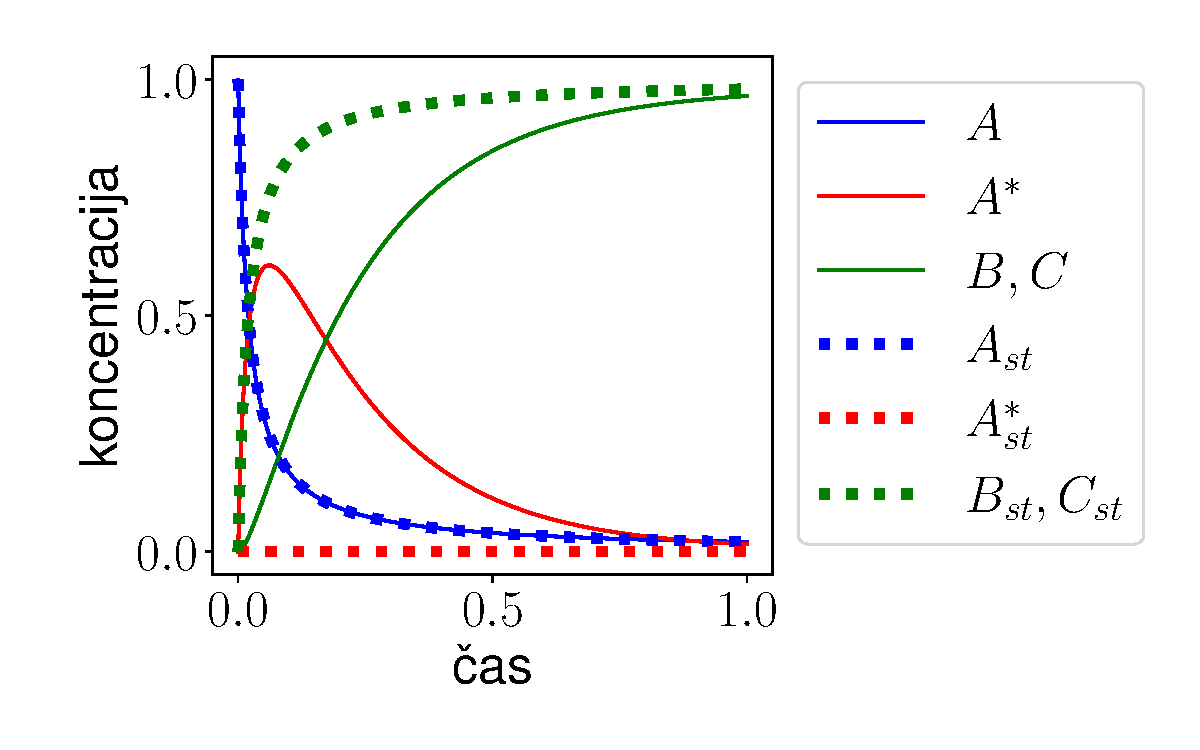
\includegraphics[width=0.5\textwidth]{5. nal slike/obratno_qp_zanimivo.pdf}
    \caption{Napaka izračuna v stacionarnem stanju pri $r/q=A(0)=1$ in spremembi $p/q= 0.001$}
    \label{fig:napaka_stacionarnega}
\end{figure}
\begin{figure} [ht!]
\begin{centering}
    \begin{subfigure}{0.3\textwidth}
        \centering
    \includegraphics[width=\linewidth]{5. nal slike/1.rq_0.1.pdf}
    \caption{$r/q = 0.1$}
    \end{subfigure}
    \begin{subfigure}{0.3\textwidth}
        \centering
    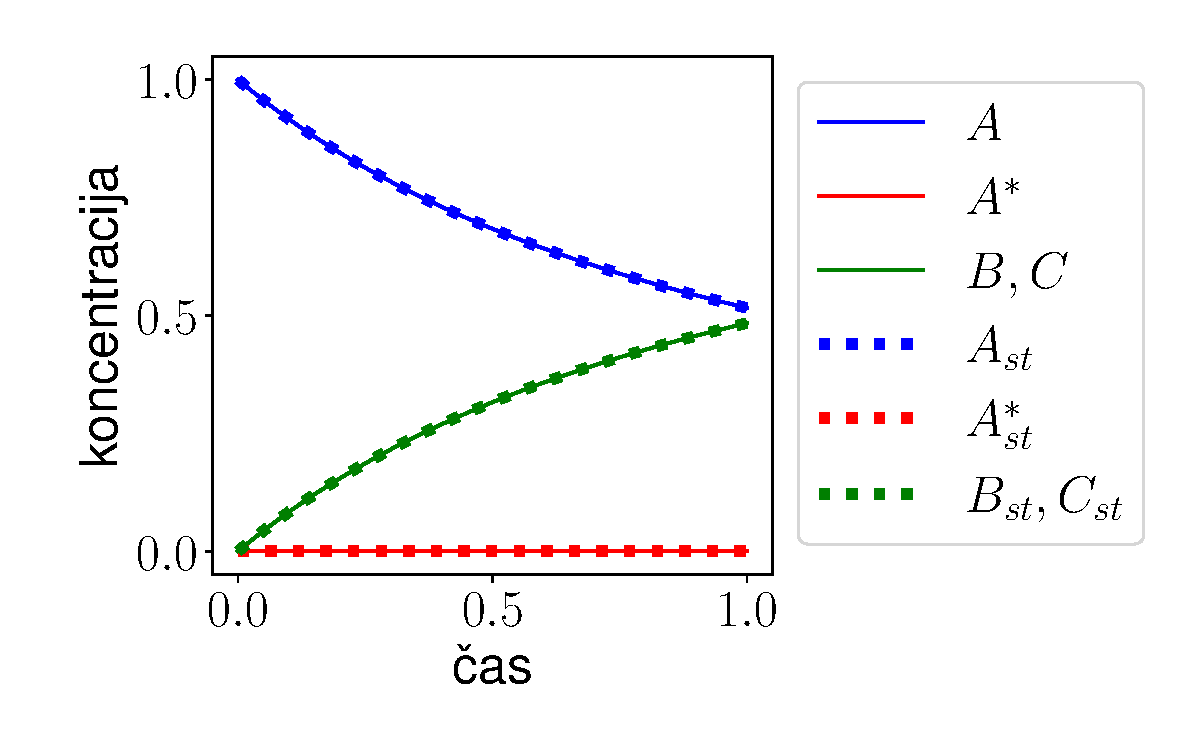
\includegraphics[width=\linewidth]{5. nal slike/1.rq_1.0.pdf}
    \caption{$r/q = 01$}
    \end{subfigure}
    \begin{subfigure}{0.3\textwidth}
        \centering
    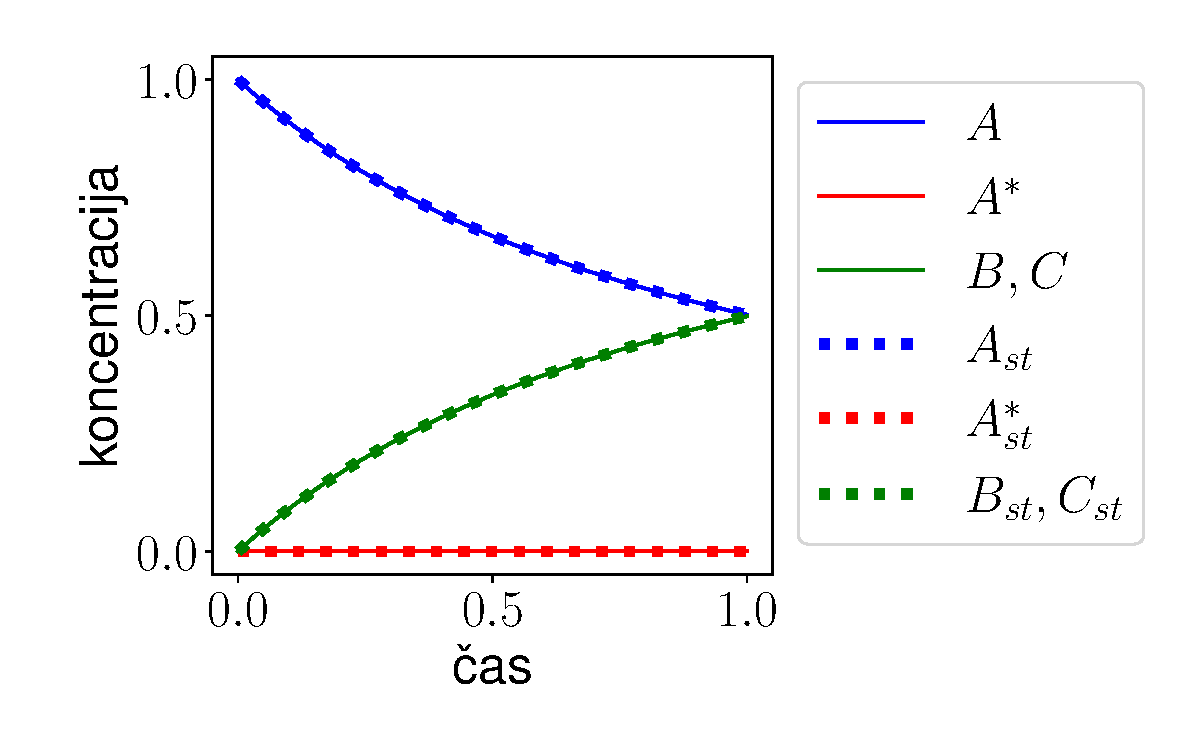
\includegraphics[width=\linewidth]{5. nal slike/1.rq_10.0.pdf}
    \caption{$r/q = 10$}
    \end{subfigure}
\end{centering}
\caption{Potek koncentracij za različne $r/q$ pri $p/q=1000$ in $A(0)=1$ in primerjava med eksaktnim izračunom in izračunom v stacionarnem stanju}
\label{fig:zahtevani_izrač}
\end{figure}
\begin{figure}[ht!]
    \centering
    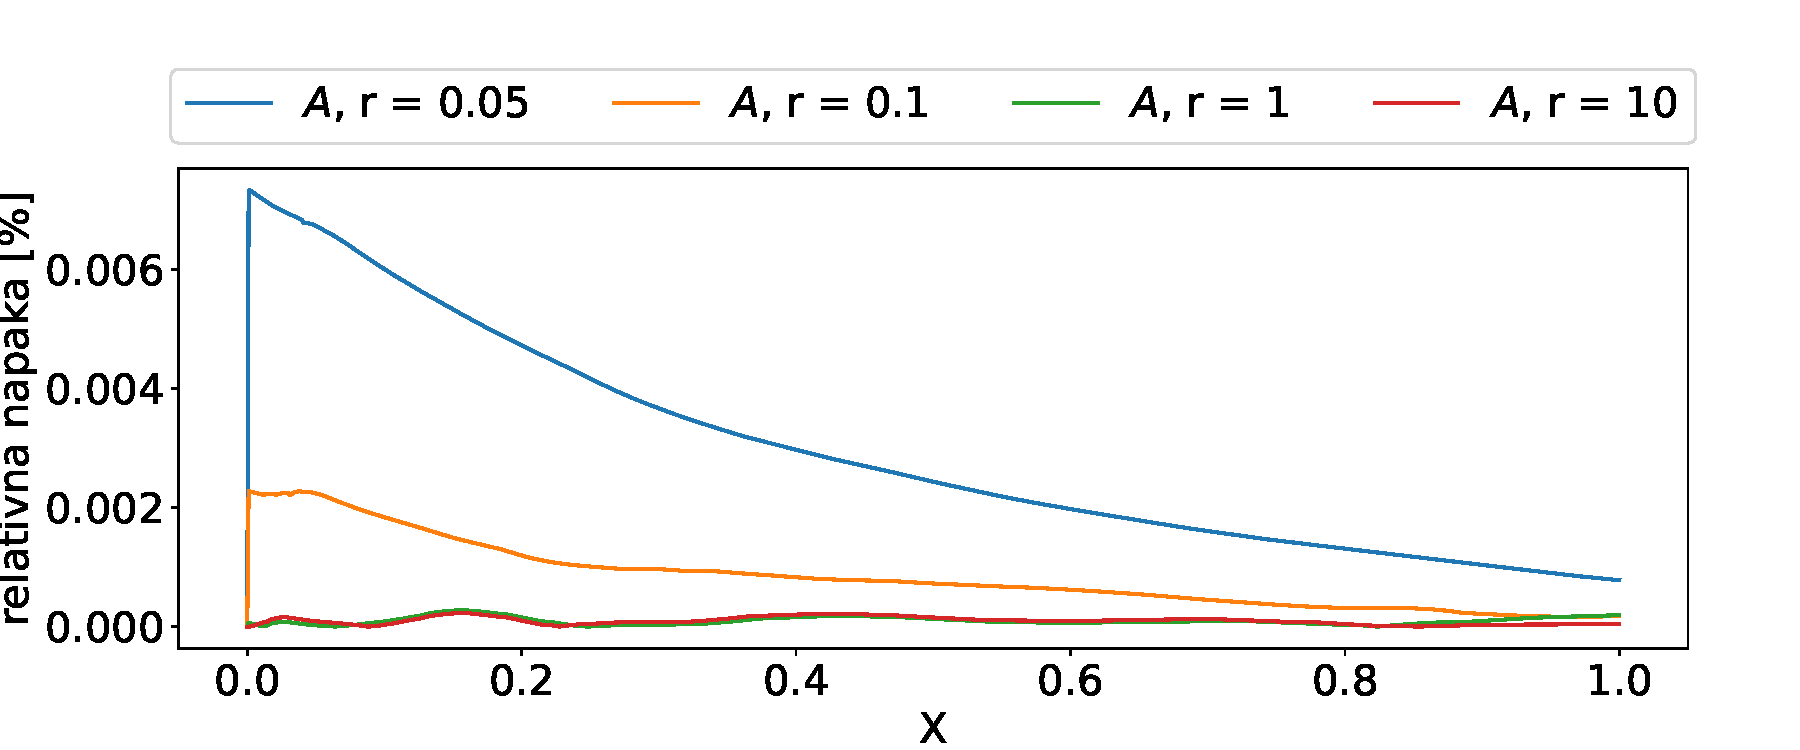
\includegraphics[width=0.6\linewidth]{5. nal slike/napaka_od_r.pdf}
    \caption{Relativna napaka aproksimacije stacionarnega stanja v primerjavi z celotno rešitvijo}
    \label{fig:napaka_r}
\end{figure}

\section{Reakcija broma}

Imamo elementarni brom, ki reagira s sledečimi reakcijami:
\begin{align}
    \text{Br}_2 \, &\autorightleftharpoons{p}{q} 2\,\text{Br} \\ \nonumber
    \text{Br} + \text{H}_2 \, &\autorightleftharpoons{r}{s} \,\text{HBr} + \text{H} \\ \nonumber
    \text{H} + \text{Br}_2 \, &\autorightarrow{t}{} \, \text{HBr} + \text{Br}
\end{align}

Kinetiko poteka reakcij opišemo s sledečim sistemom NDE:
\begin{align}
    \dot{[\text{Br}_2]} &= q\,[\text{Br}]^2 - p\,[\text{Br}_2] - t\,[\text{H}]\,[\text{Br}_2] \\ \nonumber
    \dot{[\text{H}_2]} &= s \, [\text{H}] \, [\text{HBr}] - r \, [\text{Br}] \, [\text{H}_2] \\ \nonumber
    \dot{[\text{HBr}]} &= r\,[\text{Br}]\,[\text{H}_2] - s\,[\text{HBr}]\,[\text{H}] + t\,[\text{H}]\,[\text{Br}_2]\\ \nonumber
    \dot{[\text{Br}]} &= 2\,p\,[\text{Br}_2] - q\,[\text{Br}]^2 + s\,[\text{HBr}]\,[\text{H}] - r\,[\text{Br}]\,[\text{H}_2] + t\,[\text{H}]\,[\text{Br}_2]\\ \nonumber
    \dot{[\text{H}]} &= r\,[\text{Br}]\,[\text{H}_2] - s\,[\text{HBr}]\,[\text{H}] - t\,[\text{H}]\,[\text{Br}_2]
\end{align}

Ob aproksimaciji stacionarnega stanja lahko iz enačb
\begin{align}
    \dot{[\text{Br}]} &= 2\,p\,[\text{Br}_2] - q\,[\text{Br}]^2 + s\,[\text{HBr}]\,[\text{H}] - r\,[\text{Br}]\,[\text{H}_2] + t\,[\text{H}]\,[\text{Br}_2] \approx 0 \\ \nonumber
    \dot{[\text{H}]} &= r\,[\text{Br}]\,[\text{H}_2] - s\,[\text{HBr}]\,[\text{H}] - t\,[\text{H}]\,[\text{Br}_2] \approx 0 
\end{align}
enostavno izrazimo obe neznanki $[\text{Br}]$ in $[\text{H}]$, kjer zaradi kvadratnega člena [Br] upoštevamo pozitivno vrednost koncentracij. Tako pridobimo sledeč izraz za hitrost spremembe koncentracije [HBr]:
\begin{equation}
    \dot{[\text{HBr}]} = \frac{ \frac{2\, r\, t}{s} \, \sqrt{\frac{2\,p}{q}} \, \sqrt{[\text{Br}_2]} \, [\text{H}_2]}{ \frac{t}{s} + \frac{[\text{HBr}]}{[\text{Br}_2]}}
\end{equation}

Pri primerjavi z empirično formulo
\begin{equation}
    \dot{[\text{HBr}]} = \frac{ k \, \sqrt{[\text{Br}_2]} \, [\text{H}_2]}{ m + \frac{[\text{HBr}]}{[\text{Br}_2]}}
\end{equation}
ugotovimo, da v našem primeru konstanti znašata:
\begin{equation}
    k = \frac{2\, r\, t}{s} \, \sqrt{\frac{2\,p}{q}}\text{,} \quad m =  \frac{t}{s}
\end{equation}

Tako lahko zapišemo nove proste parametre problema ($p \text{, } q \text{, } s \text{, } k \text{, } m$), saj se $t$ in $r$ lahko izrazita preko njih:
\begin{equation}
    t = m\,s \text{,}\quad r = \frac{k}{2\,m}\,\sqrt{\frac{q}{2p}}
\end{equation}
Z uvedbo novega parametra -- razmerja koncentracij med $R = \frac{[\text{H}_2]}{[\text{Br}_2]}$, popišemo začetno stanje ob predpostavki, da je vsota vseh koncentracij enaka 0.
\begin{figure}[ht!]
\begin{centering}
    \begin{subfigure}{0.5\textwidth}
        \centering
        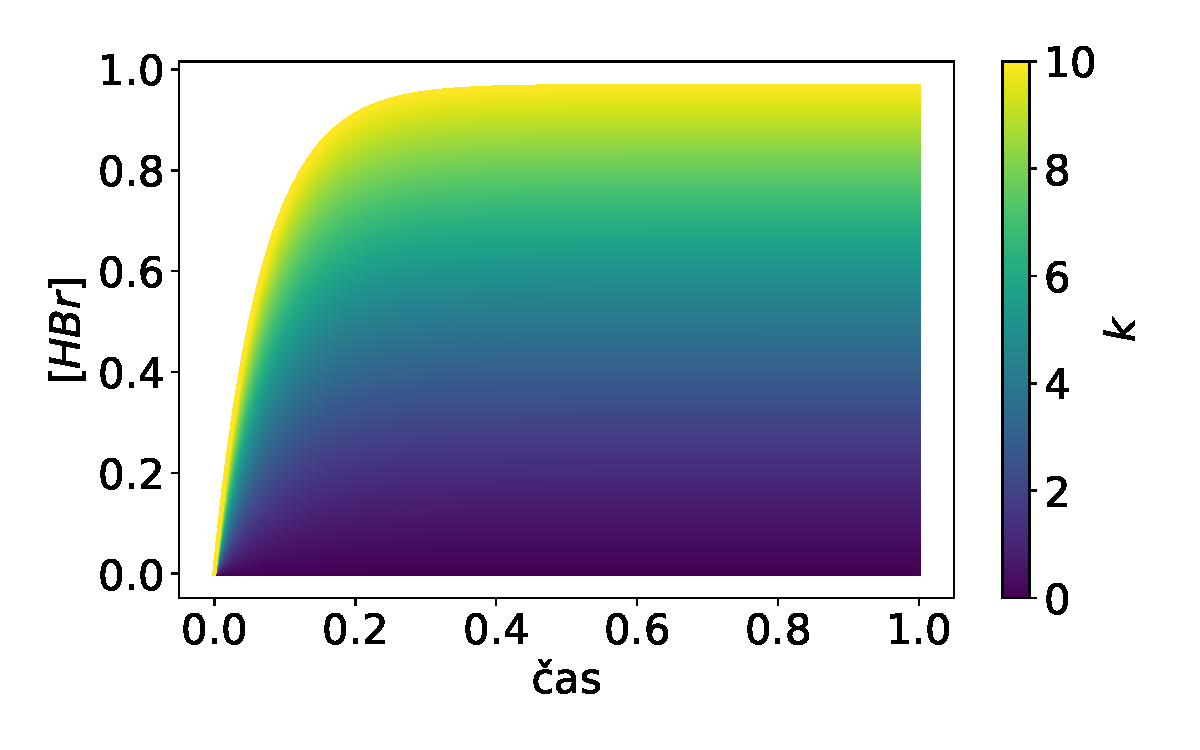
\includegraphics[width=\linewidth]{5. nal slike/potek_HBr_od_k.pdf}
        \caption{Pri $m=2.5$ in različnih parametrih $k$}
        \label{fig:HBr_od_k}
    \end{subfigure}
    \begin{subfigure}{0.5\textwidth}
        \centering
        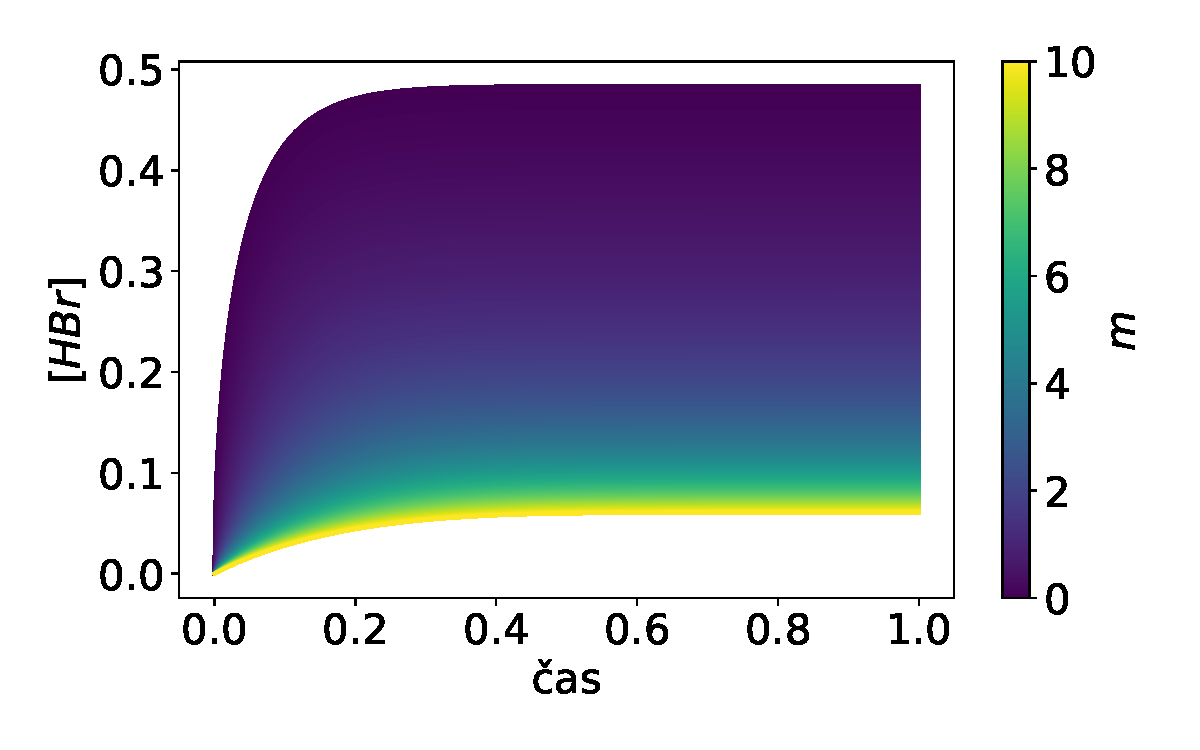
\includegraphics[width=\linewidth]{5. nal slike/potek_HBr_od_m.pdf}
        \caption{Pri $k=1$, in različnih parametrih $m$}
        \label{fig:HBr_od_m}
    \end{subfigure}
\end{centering}
\caption{Potek koncentracije HBr pri $[\text{HBr}]_0=0$ in $R=1$ }
\end{figure}

\begin{figure}[ht!]
\begin{centering}
    \begin{subfigure}{0.5\textwidth}
        \centering
        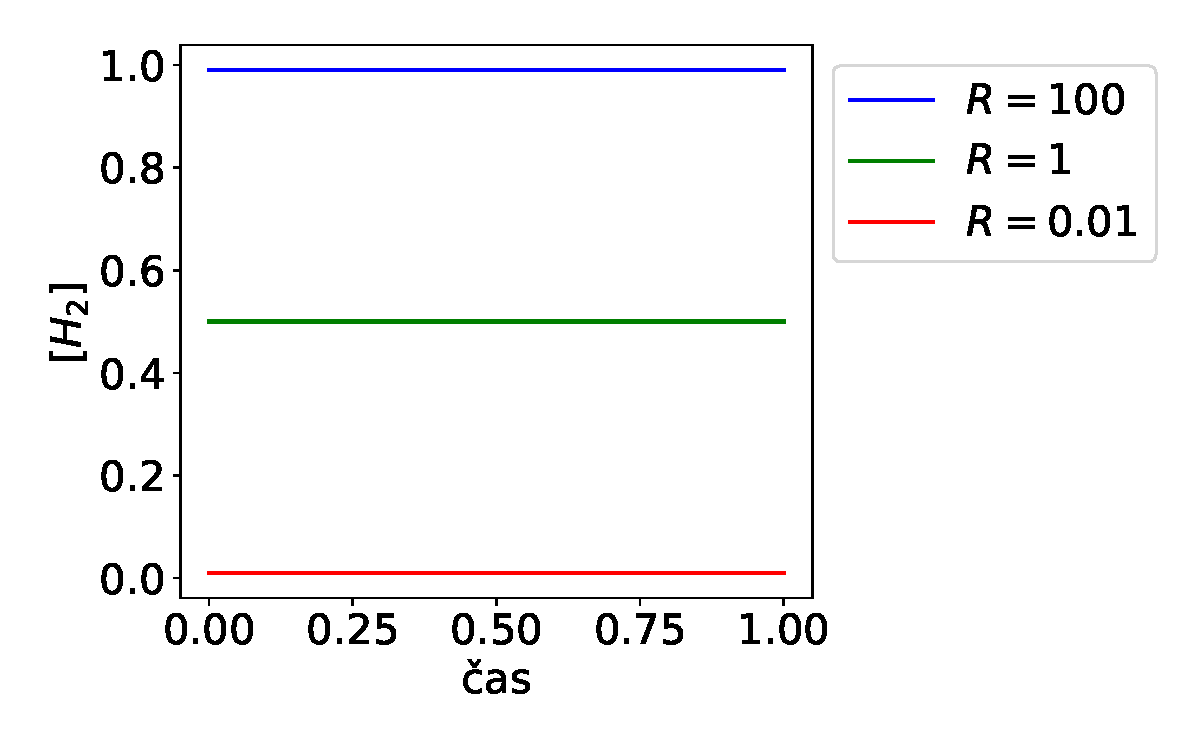
\includegraphics[width=\linewidth]{5. nal slike/potek_H2.pdf}
    \end{subfigure}
    \begin{subfigure}{0.5\textwidth}
        \centering
        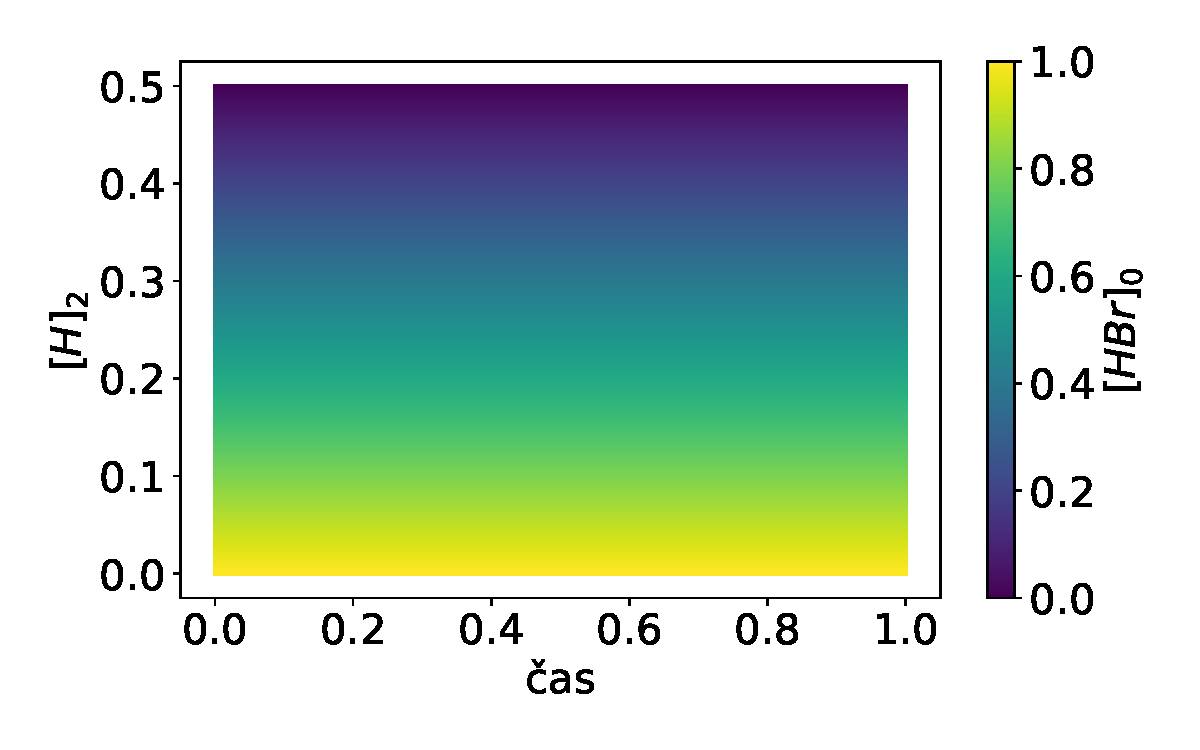
\includegraphics[width=\linewidth]{5. nal slike/potek_H2_od_HBr0.pdf}
    \end{subfigure}
    \begin{subfigure}{0.5\textwidth}
        \centering
        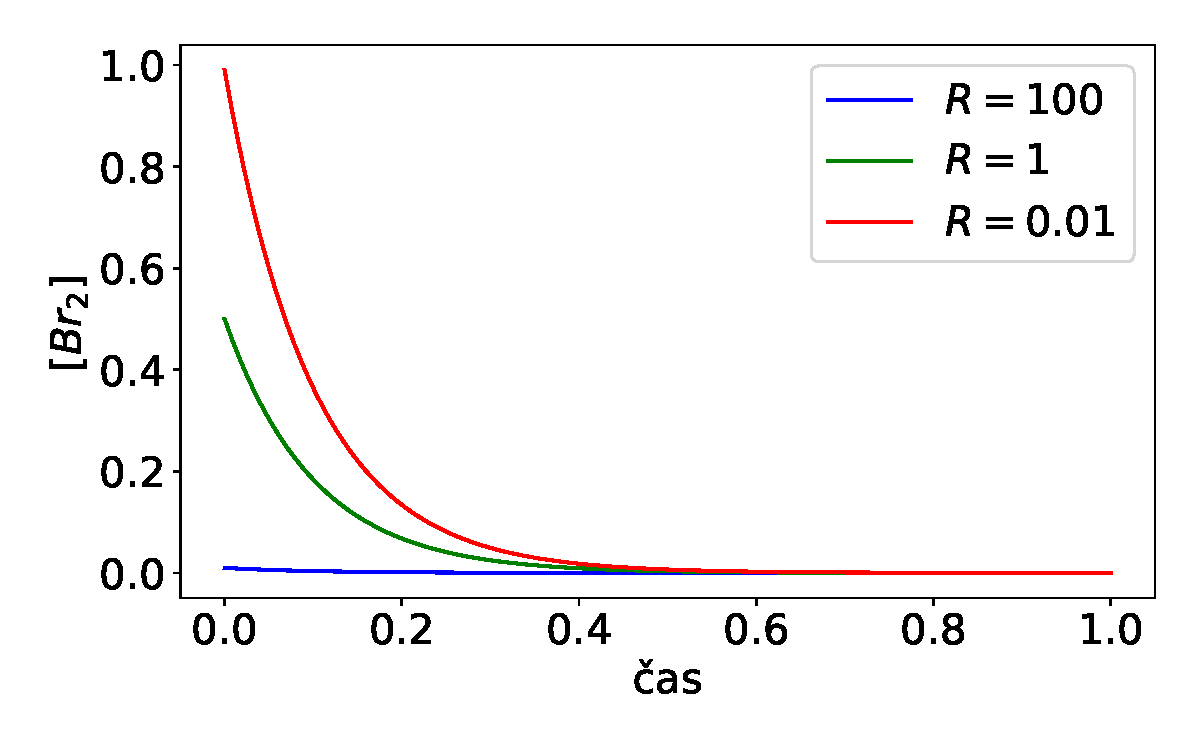
\includegraphics[width=\linewidth]{5. nal slike/potek_Br2.pdf}
    \end{subfigure}
    \begin{subfigure}{0.5\textwidth}
        \centering
        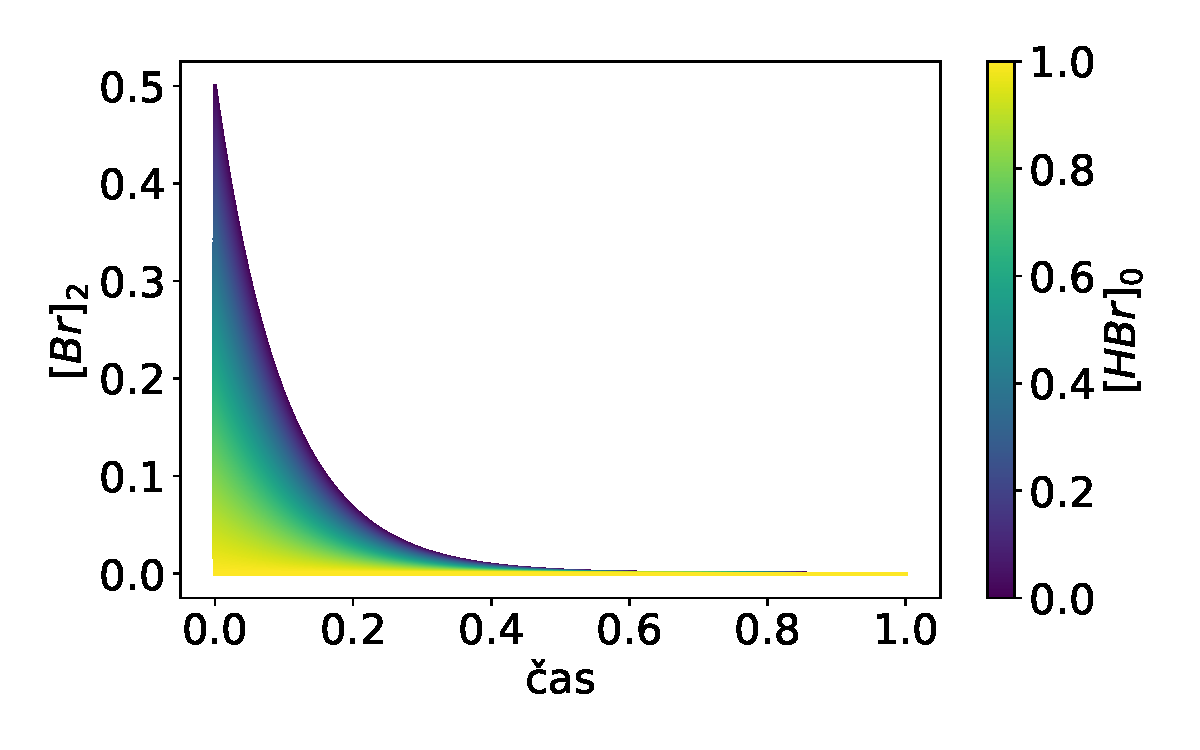
\includegraphics[width=\linewidth]{5. nal slike/potek_Br2_od_HBr0.pdf}
    \end{subfigure}
    \begin{subfigure}{0.5\textwidth}
        \centering
        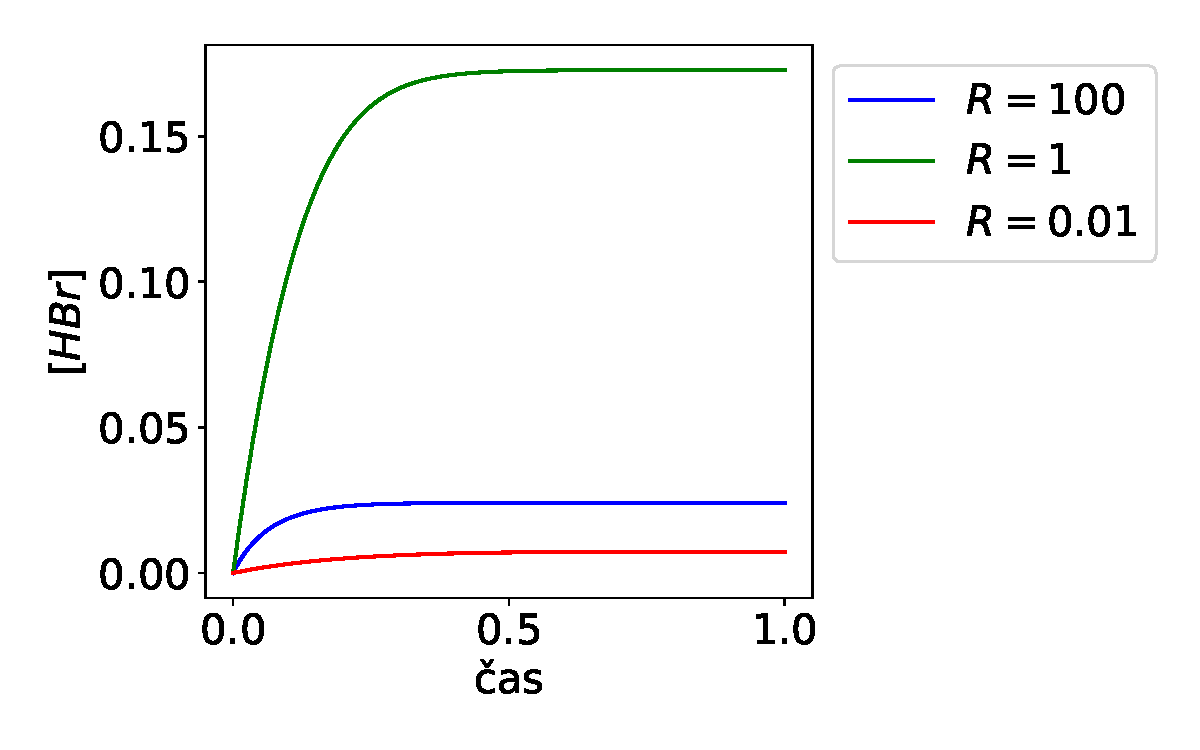
\includegraphics[width=\linewidth]{5. nal slike/potek_HBr.pdf}
    \end{subfigure}
    \begin{subfigure}{0.5\textwidth}
        \centering
        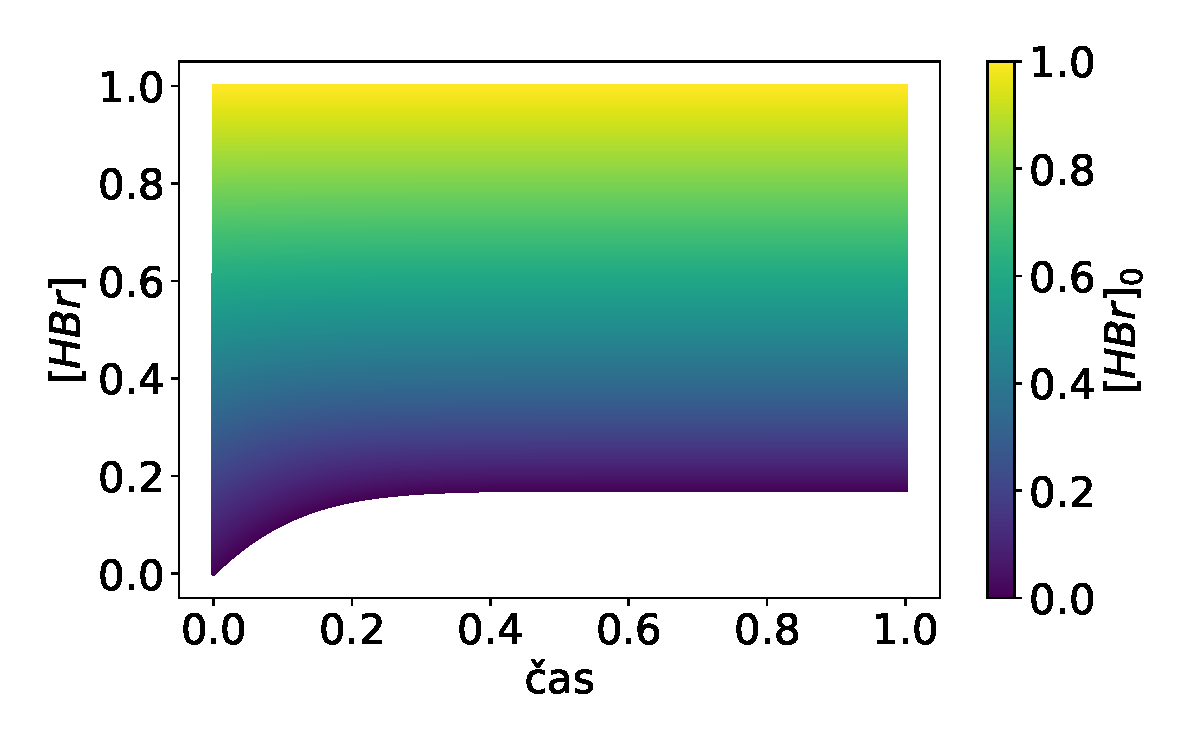
\includegraphics[width=\linewidth]{5. nal slike/potek_HBr_začetne_konc.pdf}
    \end{subfigure}
\end{centering}
\caption{Poteki koncentracij pri $m=2.5$, $k=1$, $[\text{HBr}]_0=0$ in $R=100,1,0.01$ (levo) ter $R=1$ in $[\text{HBr}]_0= (0,1)$ (desno)}
\end{figure}

\section{Jodova ura}

Tako zvane kemijske ure so reakcije, ki stečejo hitro, vendar s pričakovanim časovnim zamikom. Primer tega je jodova ura, ki sestoji iz dvoje glavnih reakcij, kjer je prva počasna, druga pa hitra. Obe sestojita iz dveh stopenj.
\begin{align}
    \text{S}_2\text{O}_8^{2-} + 2\, \text{I}^- \, &\autorightarrow{počasi}{} \, \text{I}_2 + 2\,\text{S}\text{O}_4^{2-} & 
    2\,\text{S}_2\text{O}_3^{2-} + \text{I}_2 \, &\autorightarrow{hitro}{} \, 2\,\text{I}^- + \text{S}_4\text{O}_6^{2-} \\
    \text{S}_2\text{O}_3^{2-} + \text{I}^- \, &\autorightarrow{p}{} \, \text{I}\text{S}_2\text{O}_8^{3-} & 
    \text{S}_2\text{O}_3^{2-} + \text{I}_2 \, &\autorightarrow{r}{} \, \text{I}\text{S}_2\text{O}_3^{-} + \text{I}^- \\ \nonumber
    \text{I}\text{S}_2\text{O}_8^{3-} + \text{I}^- \, &\autorightarrow{q}{} \,  \text{I}_2 + 2\,\text{S}\text{O}_4^{2-} &
    \text{I}\text{S}_2\text{O}_3^{-} + \text{S}_2\text{O}_3^{2-} \, &\autorightarrow{s}{} \, \text{I}^- + \text{S}_4\text{O}_6^{2-}
\end{align}

V približku stacionarnega stanja, ko $q >> p$ in $s>>r$, velja $\dot{[\text{I}\text{S}_2\text{O}_3^{-}]} \approx0$ in $\dot{[\text{I}\text{S}_2\text{O}_8^{3-}]}\approx0$. Pri tem uporabimo spodnjo notacijo, zapis v \textcolor{blue}{modrem} velja za hitrejšo reakcijo. Tako izpeljemo sledeče izraze za kemijsko kinetiko.
\begin{align}
    A&=\text{S}_2\text{O}_8^{2-} &
    B&=\text{I}^- &
    C&=\text{I}\text{S}_2\text{O}_8^{3-} &
    D&=\text{I}_2 &
    E&=\text{S}\text{O}_4^{2-} \\ \nonumber
    F&=\text{S}_2\text{O}_3^{2-} &
    G&=\text{I}\text{S}_2\text{O}_3^{-} &
    H&=\text{S}_4\text{O}_6^{2-}
\end{align}
\begin{align}
    \dot{A} &= -p\,A\,B \\ \nonumber
    \dot{B} &= -p\,A\,B - q\,C\,B \,\textcolor{blue}{ + \,r\,F\,D + s\,G\,F} \\ \nonumber
    0 \approx \dot{C} &= p\,A\,B - q\,C\,B \quad \chemarrow \quad p\,A\,B = q\,C\,B \\ \nonumber
    \dot{D} &= q\,C\,B \, \textcolor{blue}{-\,r\,F\,D} \\ \nonumber
    \dot{E} &= 2\,q\,C\,B \\ \nonumber
    \dot{F} &= \textcolor{blue}{ -r\,F\,D - s\,G\,F} \\ \nonumber
    0 \approx \dot{G} &= \textcolor{blue}{r\,F\,D - s\,G\,F} \quad \chemarrow \quad r\,F\,D = s\,G\,F \\ \nonumber
    \dot{H} &= \textcolor{blue}{s\,G\,F}
\end{align}
Upoštevajoč izpeljane zveze iz predpostavke stacionarnega stanja in vedenja, da komponenti $E=\text{S}\text{O}_4^{2-}$ in $H=\text{S}_4\text{O}_6^{2-}$ ne vplivata na potek reakcij, saj v njih nastopata le kot produkta, dobimo poenostavljen sistem NDE, ki opisuje hitrosti reakcij z dvema parametroma $p$ in $r$. Sistem lahko še dodatno poenostavimo z deljenjem z $r$. Pri tem uvedemo nov parameter $\lambda = r/p$, ki predstavlja razmerje hitrosti glavnih reakcij in je tako edini prosti parameter problema. Velja, da $\lambda >0$, saj je druga reakcija hitrejša od prve.
\begin{align}
    \dot{A}=\dot{[\text{S}_2\text{O}_8^{2-}]} &= -A\,B \\ \nonumber
    \dot{B}=\dot{[\text{I}^-]} &= -2\,A\,B + 2\,\lambda\,F\,D \\ \nonumber
    \dot{D}=\dot{[\text{I}_2]} &= A\,B -\lambda\,F\,D \\ \nonumber
    \dot{F}=\dot{[\text{S}_2\text{O}_3^{2-}]} &= -2\,\lambda\,F\,D
\end{align}

Pri tem opazimo, da snovi $A$ in $F$ nastopata le kot reaktanta in se tako reakcije porabljata, zato morata biti prisotna na začetku v ustrezni koncentraciji, saj vplivata na tvorjenje spojin z jodom. Sledeči sliki prikazujeta poteke koncentracij pri različnih parametrih. Pričakovano večanje začetne koncentracije $[\text{S}_2\text{O}_3^{2-}]_0$ zvišuje hitrost reakcije, medtem ko  $\lambda$ zamika potek.

Zanimivo je, da v primeru povečevanja le koncentracije tiosulfata, reakcija ne steče, če pa povečujemo koncentracijo persulfata, pa pospešimo reakcijo. To je razvidno tudi iz slike \ref{fig:čas_reakc}, kjer na sliki (b) vidimo vrh, katerega vzrok nam ni znan. Morebiti gre za numerično zadevo.

Na sliki \ref{fig:stac_nestac} je opazno, da pri enakih parametrih in enakih začetnih koncentracijah rešitvi precej odstopata. Vendar pa se rešitvi približujeta če povečujemo parametre tako, da zadostimo pogojem aproksimacije ($q >> p$, $s>>r$). Zato uvedemo nova parametra $r_1 = q/p $ in $r_2=s/r$, in pri zelo velikim vrednosti (reda velikosti $10^6$) pride do željenega skoka koncentracije $\text{I}_2$. Ker so bile reakcije zelo različnih hitrosti, algoritem \texttt{LSODA} ni bil dovolj učinkovit in vrne drugačne rezultate, zato sem uporabljal bolj togega \texttt{BDF}. Očitno je, da v primeru povečevanja $\lambda$ skok postaja bolj strm. Iz tega lahko sklepamo, da smo z nestacionarno reakcijo bolje popisali sistem.

\begin{figure}[ht!]
    \centering
    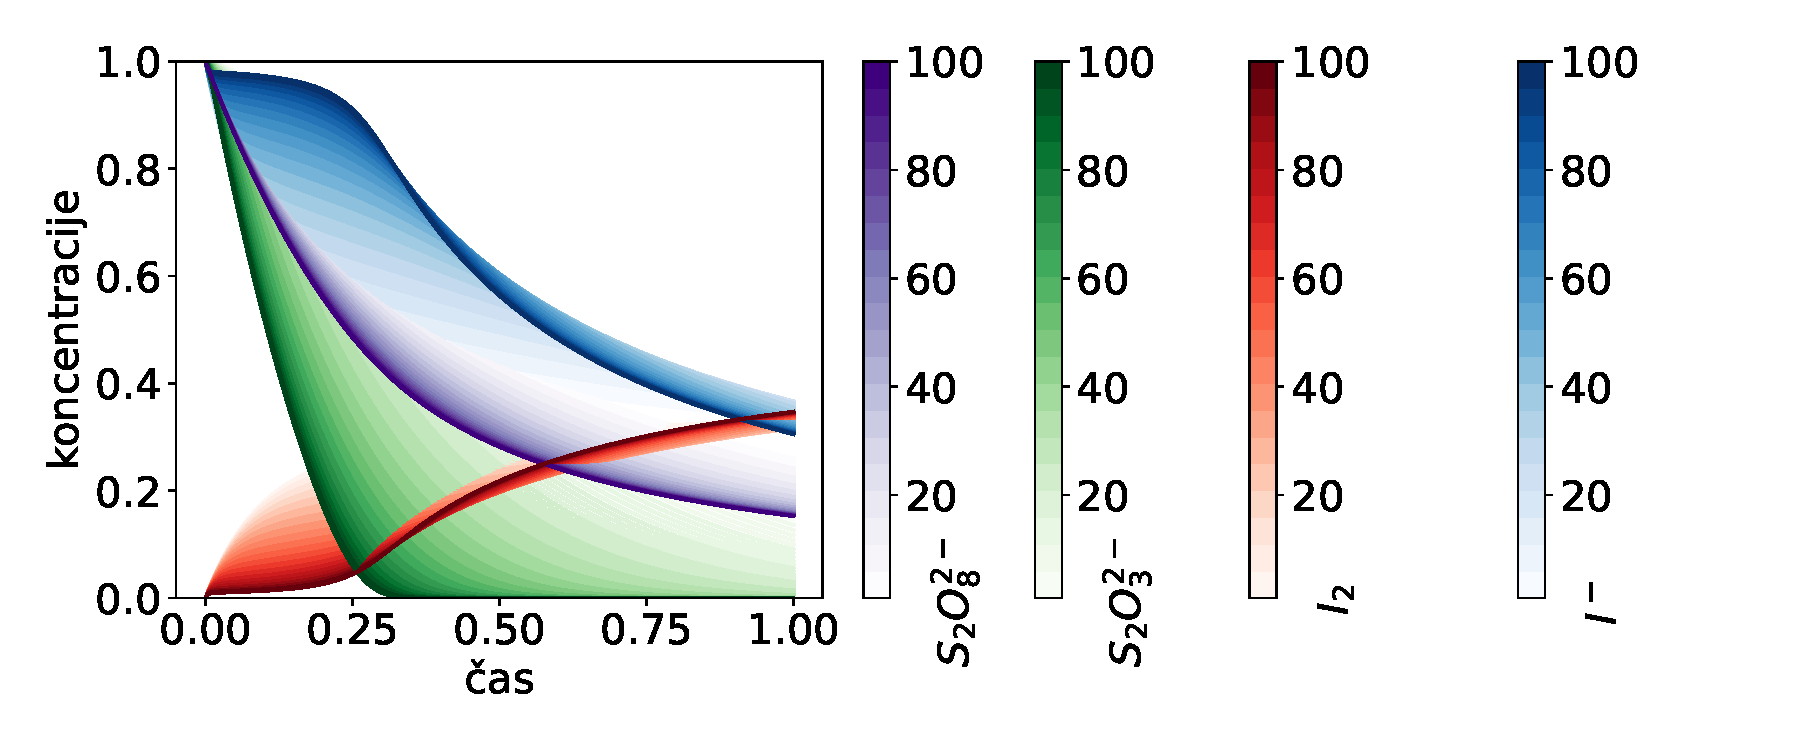
\includegraphics[width=\linewidth]{5. nal slike/jod_lambda.pdf}
    \caption{Potek koncentracij komponent za $\lambda \, \epsilon \,  (0,100)$}
\end{figure}
\begin{figure}[ht!]
    \centering
    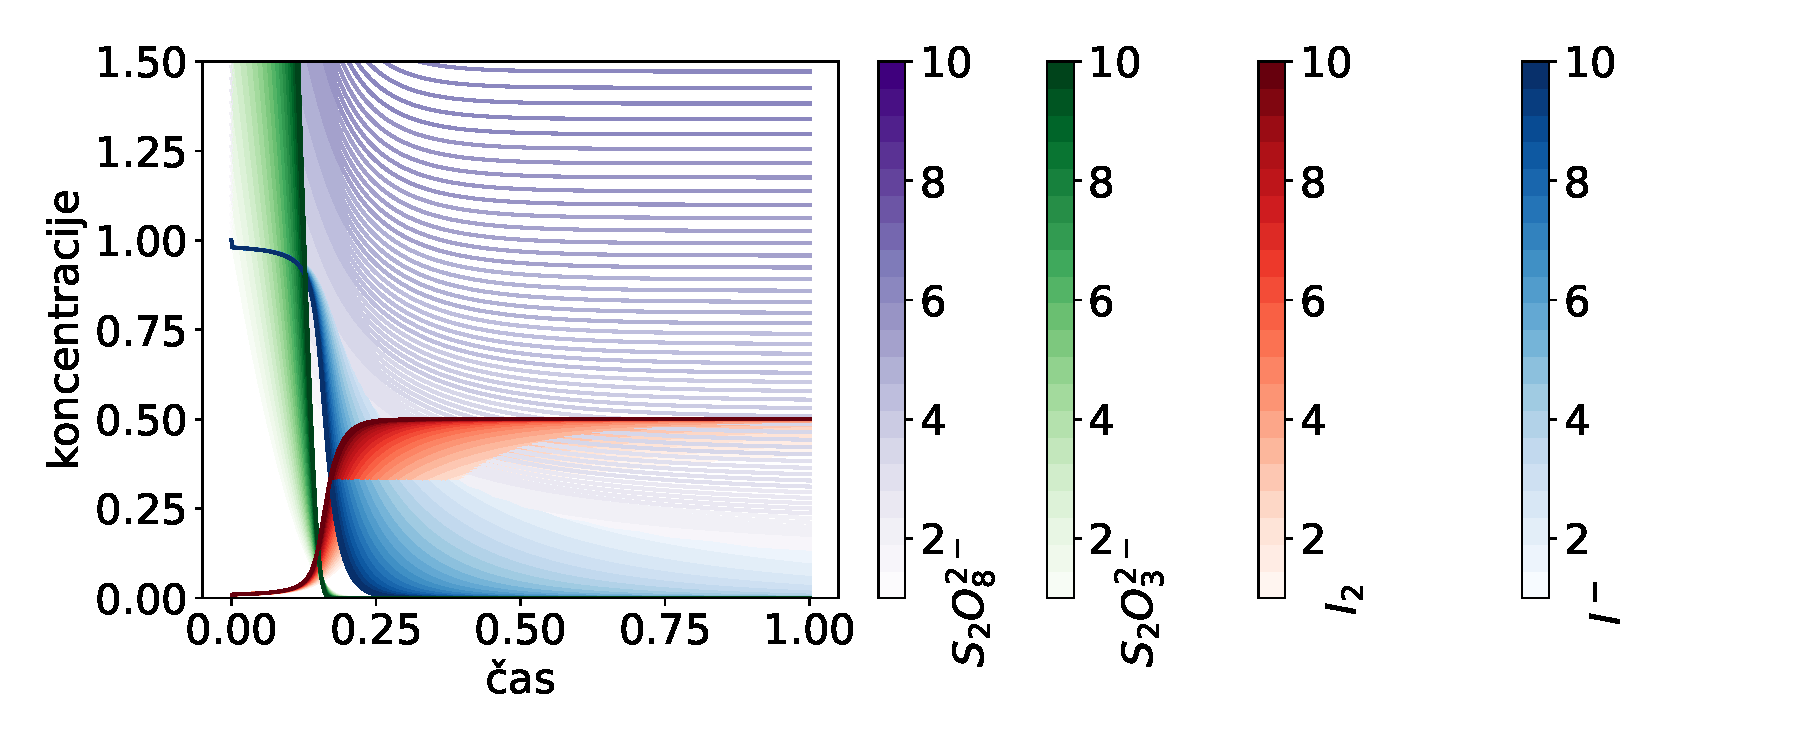
\includegraphics[width=\linewidth]{5. nal slike/jod_konc_F.pdf}
    \caption{Potek koncentracij komponent za začetno koncentracijo tiosulfata enako persulfatu $[\text{S}_2\text{O}_8^{2-}]_0 = [\text{S}_2\text{O}_3^{2-}]_0 \,  \epsilon \, (0, 10)$}
\end{figure}

\begin{figure}[ht!]
\begin{centering}
    \begin{subfigure}{0.5\textwidth}
        \centering
        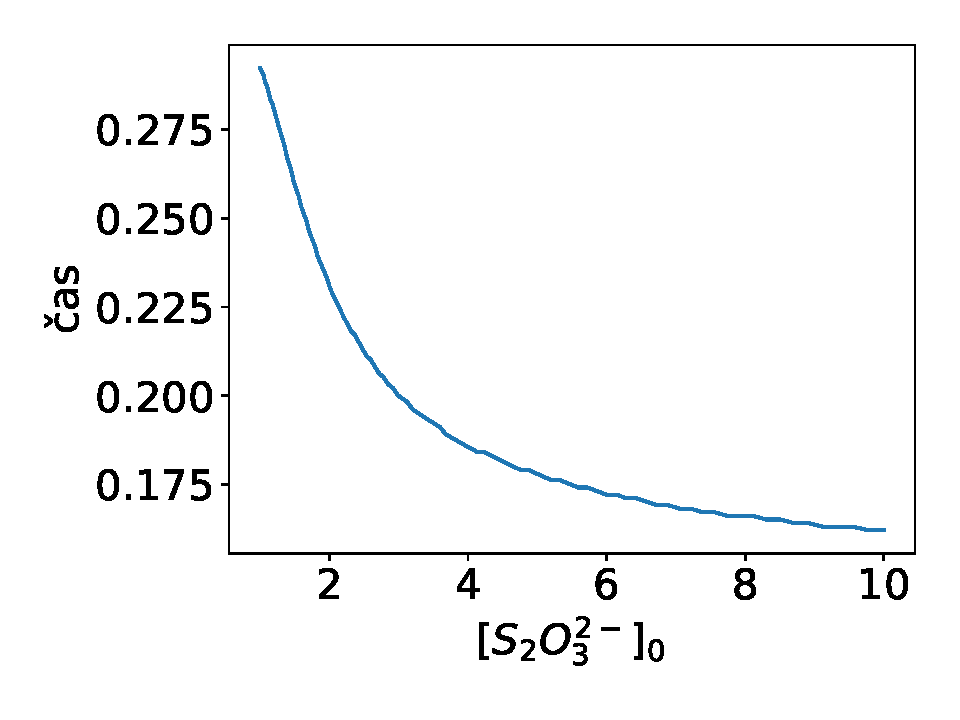
\includegraphics[width=\linewidth]{5. nal slike/čas_reakc_zač_konc.pdf}
        \caption{Odvisnost sredinskega časa reakcije od začetne koncentracije $[\text{S}_2\text{O}_3^{2-}]_0$}
    \end{subfigure}
    \begin{subfigure}{0.5\textwidth}
        \centering
        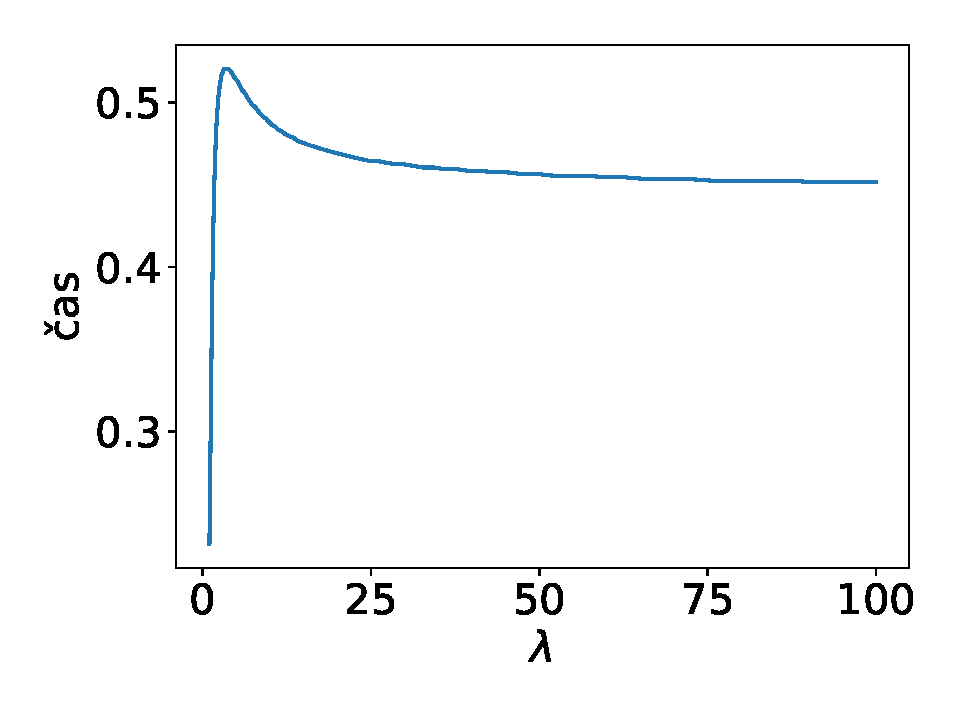
\includegraphics[width=\linewidth]{5. nal slike/čas_reakc_lambda.pdf}
        \caption{Odvisnost sredinskega časa reakcije od parametra $\lambda$}
    \end{subfigure}
\end{centering}
\caption{Čas nastopa reakcije je določen kot čas, koncentracija $\text{I}_2$ doseže svojo polovično vrednost glede na stabilno stanje}
\label{fig:čas_reakc}
\end{figure}

\begin{figure}[ht!]
\begin{centering}
    \begin{subfigure}{\textwidth}
        \centering
        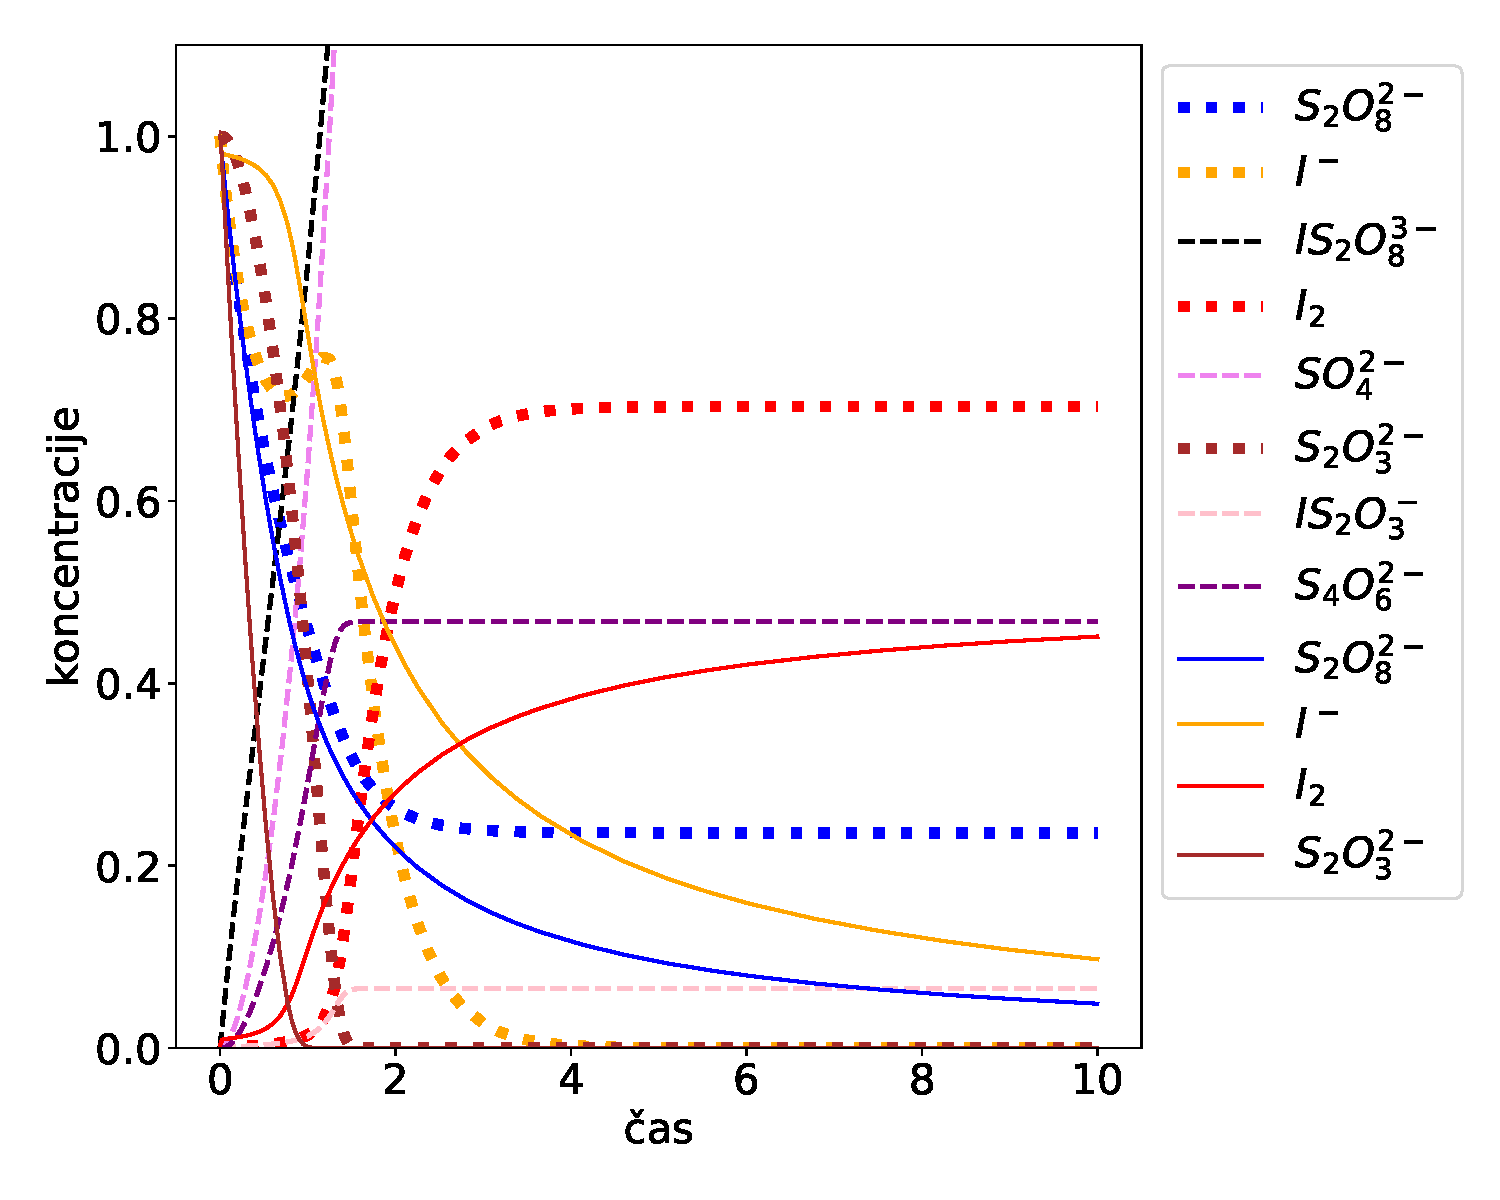
\includegraphics[width=0.65\linewidth]{5. nal slike/stac_nestac.pdf}
        \caption{$\lambda=1$, $r_1 = q/p =1$, $r_2=s/r=1$}
    \end{subfigure}
    \begin{subfigure}{\textwidth}
        \centering
        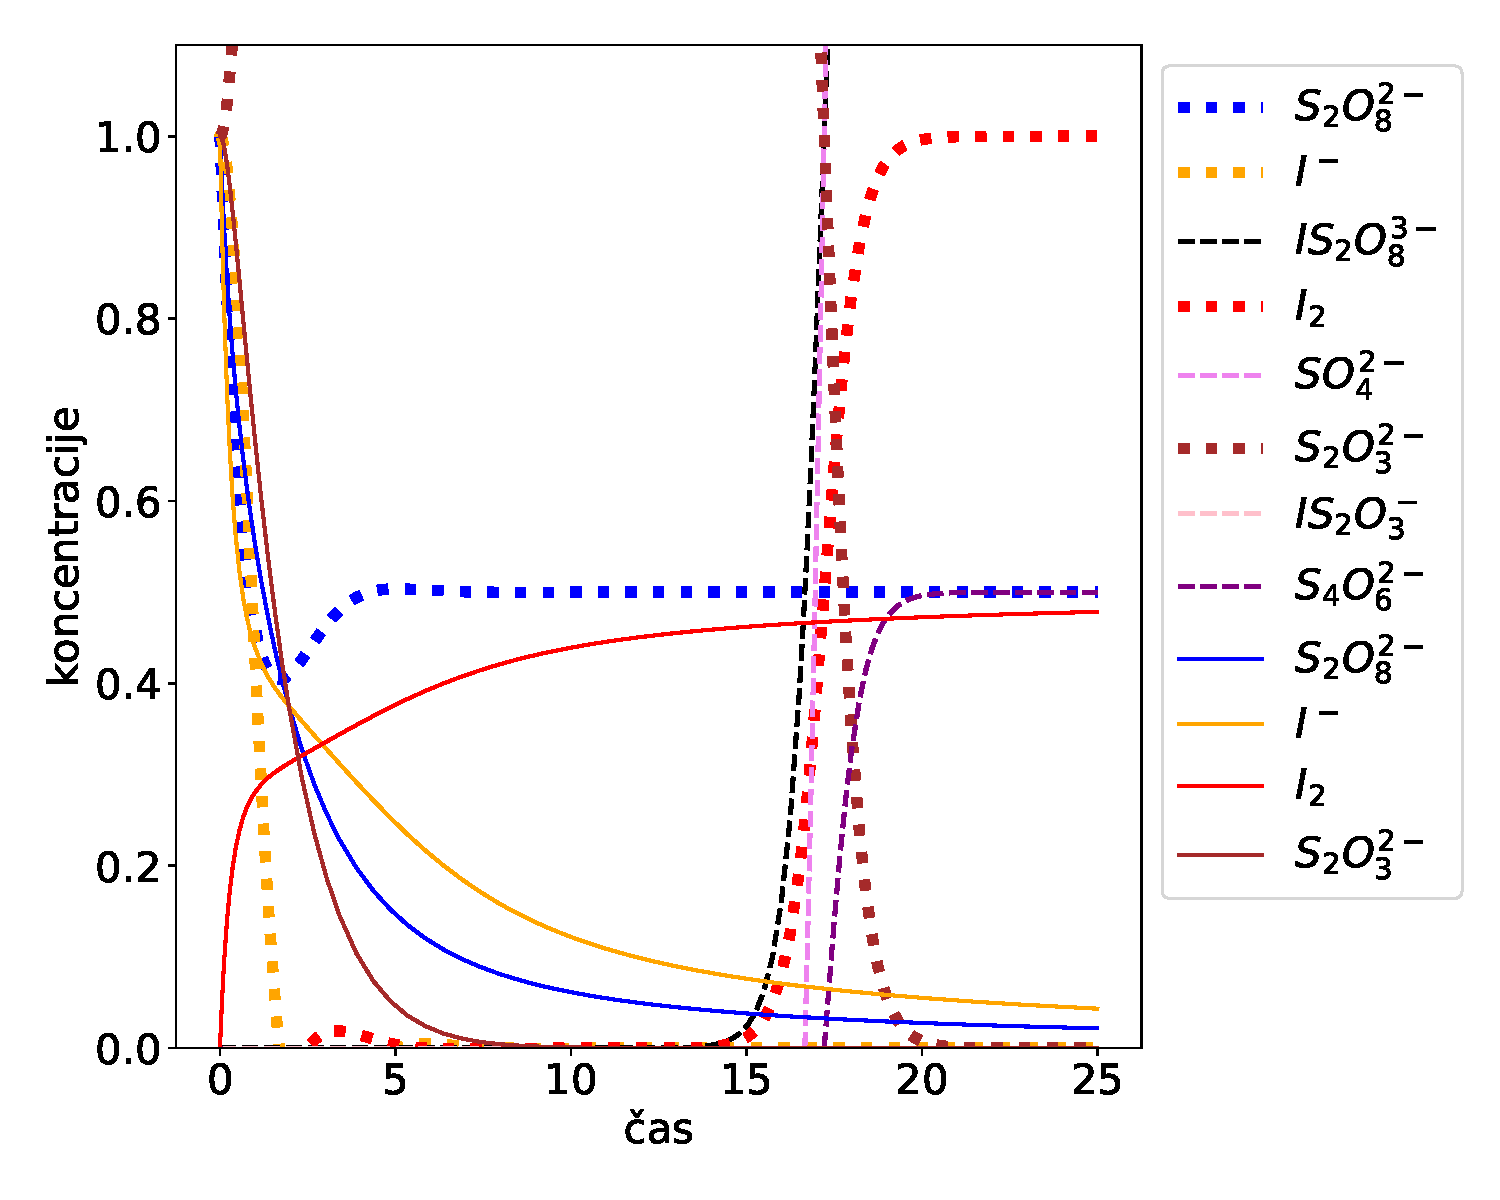
\includegraphics[width=0.65\linewidth]{5. nal slike/stac_nestac_pribl.pdf}
        \caption{$\lambda=1$, $r_1 = q/p =1$, $r_2=s/r=1$}
    \end{subfigure}
\end{centering}
\caption{Primerjava med izračunom v aproksimaciji stacionarnega stanja (debele črte) in splošnim izrazom (črtkano)}
        \label{fig:stac_nestac}
\end{figure}

\newpage
\section{Belousov–Zhabotinsky reakcija}

Sicer kompleksno reakcijo lahko popišemo s sistemom treh preprostih reakcij \cite{Turner2009_BZ_raction}, ki omogočajo krožno spremembo med spojinami A, B in C:
\begin{align}
    A+B \, &\xrightarrow{\alpha} \, 2\,A \\ \nonumber
    B+C \, &\xrightarrow{\beta} \, 2\,B \\ \nonumber
    C+A \, &\xrightarrow{\gamma} \, 2\,C
\end{align}
\begin{align} \label{eqn:B_Z_react}
    \dot{[A]} &= \alpha \, A\,B - \gamma\,A\,C \\ \nonumber
    \dot{[B]} &= \beta\,B\,C - \alpha \, A\,B \\ \nonumber
    \dot{[C]} &= \gamma \, A\,C - \beta\,B\,C 
\end{align}
Zapišemo lahko tudi zgornje enačbe sprememb koncentracij, kot do sedaj, vendar nam celokupna koncentracija ne pove, kako lokalno oscilirajo -- nastanek značilnih vzorcev. Zato moramo sistem obravnavati lokalno, za kar je uporabna metoda celičnih ali točkovnih avtomatov, kjer primer diskretiziramo in obravnavamo stanje točke glede na stanje v prejšnjem koraku in stanja sosednjih točk. Za definicijo okolice izberemo Moore-ovo okolico, kot je opisano v \cite{Turner2009_BZ_raction}, koncentracije spojin aproksimiramo:
\begin{align}
    [A]_{t+1} &= [A]_t + [A]_t \, (\alpha \,[B]_t - \gamma \,[C]_t) \\ \nonumber
    [B]_{t+1} &= [B]_t + [B]_t \, (\beta \,[B]_t - \alpha \,[A]_t) \\ \nonumber
    [C]_{t+1} &= [C]_t + [C]_t \, (\alpha \,[B]_t - \beta \,[B]_t)
\end{align}
pri čemer upoštevamo parametre $\alpha$, $\beta$ in $\gamma$ za hitrosti reakcij. Pri simulaciji upoštevamo kot koncentracijo spojine povprečno koncentracijo v obravnavani točki in okolici v prejšnjem koraku. 

Za $\alpha=0,8$ in $\beta=\gamma=1$ dobimo sledeče rezultate. Bolj nazoren prikaz je na sliki \textit{reakcija.gif} v prilogi.
\begin{figure}[ht!]
    \centering
    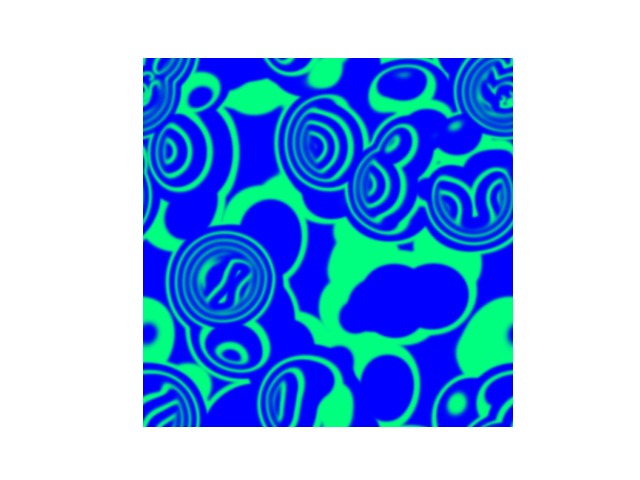
\includegraphics[width=0.7\textwidth]{5. nal slike/Figure_1.png}
    \caption{Simulacija pri naključnih začetnih pogojih koncentracij}
\end{figure}
\begin{figure}[ht!]
    \centering
    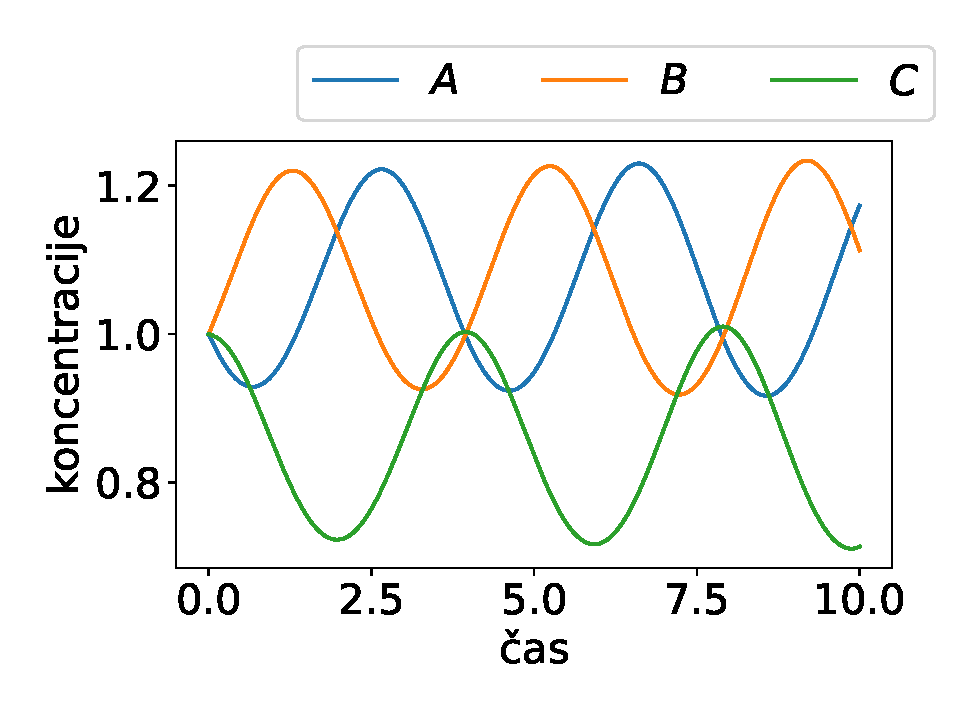
\includegraphics[width=0.5\textwidth]{5. nal slike/B_Z_konc.pdf}
    \caption{Potek oscilacij koncentracij, izračunan z integracijo enačb \ref{eqn:B_Z_react}}
\end{figure}